\chapter{Slice Testing}

The long-term goal of this work is to create an integrated biosensor for use with living cells. Thus, proof-of-concept tests were performed. This chapter describes these tests and results.

\section{Slice Information}

Mouse-ovary slices were prepared and attached by the Department of Biomedical Sciences at Colorado State University. Slices were prepared as described in \cite{tobet2003vcm}, but with changes to use ovary instead of brain slices. Those changes include: they were not cut on a specific plane and they were not plated on glass coverslips (rather, on the chips). The ovaries were sectioned at $200 \mu \mathrm{m}$ thick in adult, female mice.

\section{Experiment Procedure}

Since the slices had to be tested while alive, and thus at a temperature of $37\,^{\circ}\mathrm{C}$, we were forced to use a heating device. We chose a heat lamp, placed in the Faraday cage, next to the chip. Tests were performed using the method below (amperometry for 30 minutes), but without ovary, which showed that the lamp did not contribute noticable noise to the output.

To find the ideal potential at which to run the amperometry, a hydrodynamic voltammogram (HDV) was performed to find the optimum potential for amperometry. This was done by running multiple amperometry experiments at identical conditions except for potential, which was varied between 0.6V and 1.25V. In order to ensure identical conditions, the electrode was cleaned before each run by CV from 1.5V to -0.8V at 1V/s for 100 cycles in $\mathrm{H}_2 \mathrm{SO}_4$. The chip well was filled with 50$\mu$L 0.1M KCl. A syringe of 600$\mu$M NE was loaded into a pump. The end of the syringe was connected to a pipette, the end of which was lowered into the well so that it was below the surface of the solution. An amperometry experiment was carried out where the syringe pump would be enabled for 10 seconds at 100$\mu$L/min. The value of the experiment was taken to be the difference between the idle point just before the syringe pump was enabled (generally close to 0) and the lowest point of the resulting curve. The optimum potential was found by taking the largest result, which was at 0.85V (Figure \ref{hdv}).

\begin{figure}
	\centering
	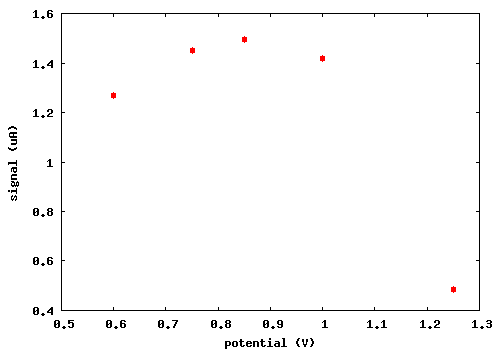
\includegraphics[width=0.7\linewidth]{figures/hdv.png}
	\caption{HDV for norepinephrine}
	\label{hdv}
\end{figure}

These tests were done by preparing a chip with the PDMS well, doing a basic CV to determine if the chip was working (although not how well it worked), and attaching a living slice of a mouse ovary to the surface of the chip, over the sensor sites. Care was taken to ensure the slice would stay living up to and during the tests by keeping it at a temperature of $37\,^{\circ}\mathrm{C}$, and submerged in neurobasal. After the ovary slice was attached the chip was moved into a different lab. The temperature was measured by lowering the end of a thermometer below the surface of the neurobasal, and heated with a lamp to the appropriate temperature (Figure \ref{slice-top}). The entire testing device was enclosed in a Faraday cage. Previously, a chip had been prepared in the same fashion, but with no ovary, and tested with the lamp on. This test showed that the lamp did not contribute noise to the results. After these preparations, the chip was connected to the 660B potentiostat at sensor 17, working electrode 41. Amperometry was performed at 0.85V for 30 minutes.

\begin{figure}
	\centering
	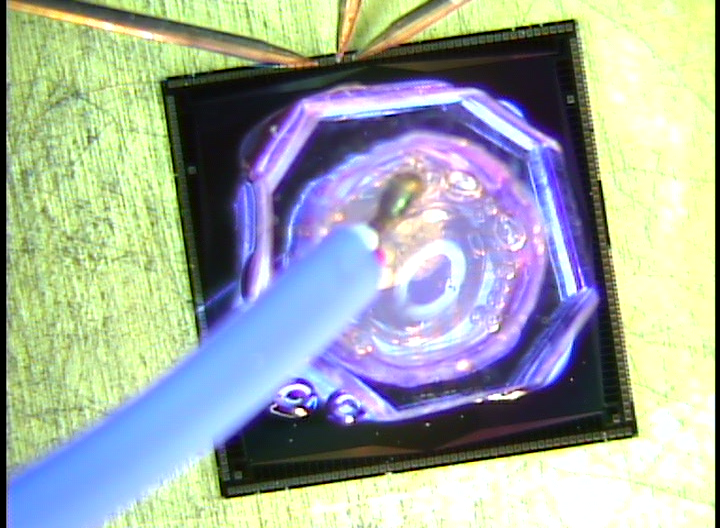
\includegraphics[width=0.5\linewidth]{figures/slice-top.png}
	\caption[Top view of chip under testing with an ovary slice attached]{Top view of chip under testing with an ovary slice attached. The blue wire is a temperature sensor.}
	\label{slice-top}
\end{figure}

\section{Experiment Results}

Figure \ref{216} shows an excerpt of a test. Thes results are consistent with the release profile: it exhibits multiple sharp changes, followed by an exponential decrease back to the baseline.

\begin{figure}
	\centering
	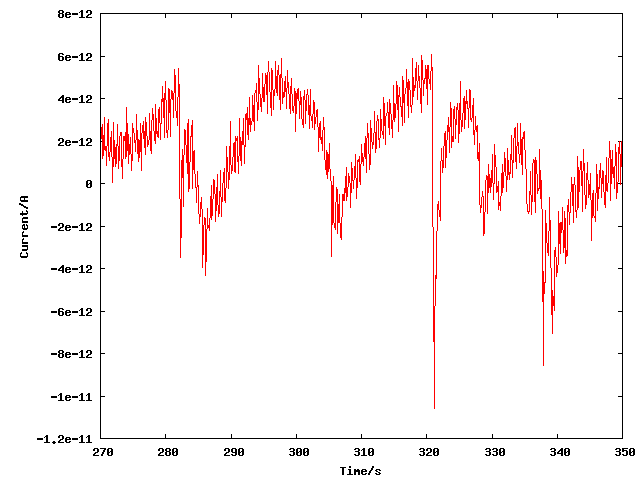
\includegraphics[width=0.7\linewidth]{figures/216.png}
	\caption{Amperometric pulses from ovary-slice test.}
	\label{216}
\end{figure}

\section{Discussion}

Figure \ref{mosharok-pulses} shows a similar test from another group. Our pulses have a longer time duration (5s compared to 50ms) and a smaller peak height (10pA compared to 100pA). However, our electrodes are much smaller, which accounts for some of these differences. It appears that our chip is able to detect chemical releases from a living cell. Hence, with the right instruments, future work could pursue obtaining a chemical gradient. This would require many electrodes being used at once, either with many potentiostats or a multi-channel potentiostat. Further work should also characterize the performance of the sensors with attached ovary slices. Currently we do not have any reliable data to show the concentrations of chemicals that are released from the cell. However, our results show proof-of-concept results.

\begin{figure}
	\centering
	\begin{tabular}{rl}
		\textbf{a} \\ & 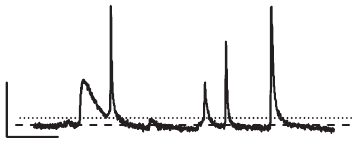
\includegraphics[width=0.5\linewidth]{figures/mosharok-pulse.png} \\
		\\
		\textbf{b} \\ & 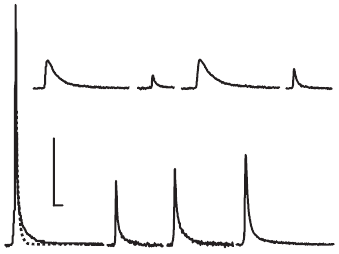
\includegraphics[width=0.5\linewidth]{figures/mosharok-pulse-2.png}
	\end{tabular}
	\caption[Amperometric pulses from another group]{Amperometric pulses from another group. (a) Figure 2 (a) of \cite{mosharok2005aee}, which used a carbon fiber electrode placed against the surface of a secretory cell. Scale bars, 50pA and 100ms for the timescale. (b) Figure 4 of \cite{mosharok2005aee}: amperometric events belonging to the same experimental trace. Scale bars, 50pA and 10ms for the timescale.}
	\label{mosharok-pulses}
\end{figure}
